\section{Load Balancing}
Load balancing refers to the concept of distributing requests between different servers in such a way that the amounts of requests per server are balanced.
It is a necessary component of a system where a single instance cannot service all requests, and thus multiple instances are used to keep performance levels acceptable.
A balanced distribution can depend on one's objectives, but typically aims to maximize overall system performance over the available servers\cite{cardelliniDynamicLoadBalancing1999a}.

While load balancer type system components are ubiquitous in our modern computing environment, in this work we focus solely on web load balancers.
From the perspective of the OSI network reference model\cite{dayOSIReferenceModel1983}, load balancers typically work on the transport layer (level 4), or the application layer (level 7).
Because serverless frameworks like OpenFaaS differentiate between functions based on HTTP request data, only application-level load balancing is of concern for us in the context of this paper.

There exist a large number of load balancing algorithms, which decide the application instances servicing each request.
The most common algorithms include:
\begin{itemize}
    \item \textbf{Round Robin:} requests are distributed evenly between servers, irrespective of the performance or load of each server. Each subsequent request is sent to a different server.
    \item \textbf{Weighted Round Robin:} requests are also distributed among servers, but not necessarily evenly. Each server is manually assigned a weight, which determines the share of requests it receives relative to other servers. Weights scale linearly, meaning that one server having double the weight of another also means that it will receive double the requests
    \item \textbf{Least Response Time:} can be implemented in different ways. In the naive approach the load balancer forwards all requests to the server showing the fastest initial response time, until that server's performance degrades to the point where another server is faster, which receives subsequent requests from that point on.
\end{itemize}

Since OpenFaaS\cite{openfaas} builds on Kubernetes and its primitives, it also delegates service resolution and thus request routing to it.
While Kubernetes can use any type of load balancer in principle, particularly the kinds available from cloud providers as a managed service, it defaults to using its internal kube-proxy to handle traffic routing, which in turn defaults to using a round robin load balancing strategy.
Next, we elaborate on the role load balancing plays in serverless frameworks in a bit more detail.


\subsection{ Definition \& Role In a Typical Serverless Framework}
To give a bit more context to the role of load balancers in this work, we now discuss what component exactly we mean by \textit{load balancer}, and how it functions in the context of a serverless framework. While our approach is not tied to any specific serverless framework, implementation, or technology, we developed it with their general concepts and functioning in mind. Because of this, we feel that is helpful and informative to explain the components of our system in the context of an actual implementation, since this helps understand the abstract role these components play. In addition, this is helpful for anyone who might want to integrate our approach into a production ready serverless edge computing platform.

As previously mentioned there are a number of different serverless frameworks, some free, some open source, some commercial, and some that fall in-between\cite{aws-lambda}\cite{azure-functions} \cite{openfaas-gateway}\cite{kubeless}\cite{openwhisk}.
To reiterate, we choose OpenFaaS as a proxy for serverless computing frameworks in general because it has been extended for edge computing, and because it builds on and makes use of well established technologies in the same way other serverless frameworks do\cite{kubeless}\cite{openwhisk}, thus making it representative for the space.


\begin{figure}
    \centering
    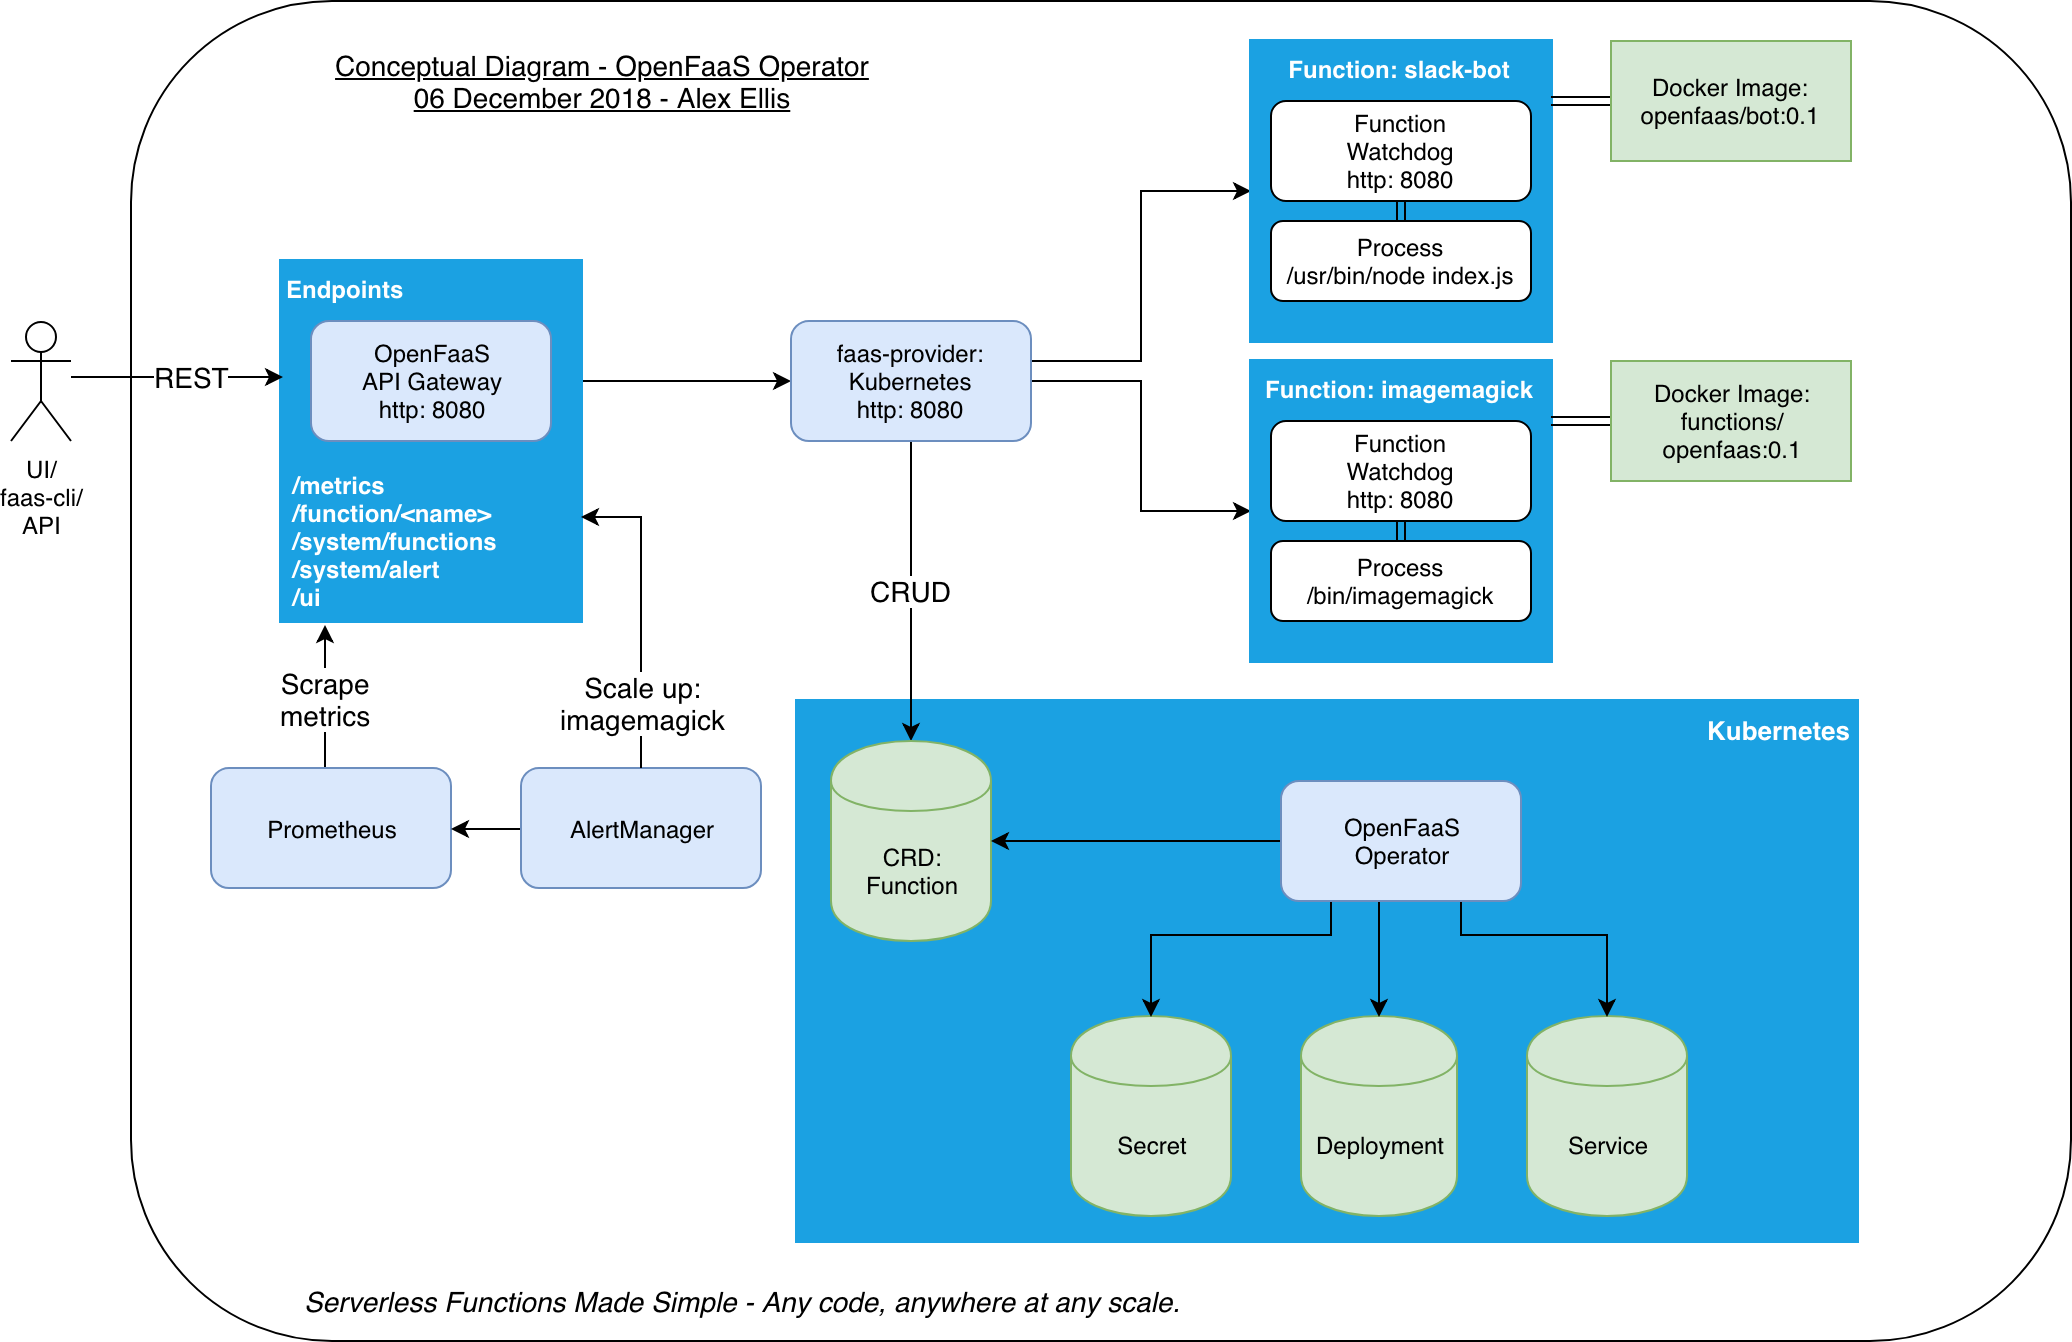
\includegraphics[width=14cm]{graphics/diagrams/openfaas-gateway-architecture.png}
    \caption{Diagram showing the architecture and components of OpenFaaS, in particular the OpenFaaS API Gateway. Taken from the official OpenFaaS architecture documentation\cite{openfaas-gateway}}
    \label{fig:openfaas-gateway-diagram}
\end{figure}


As mentioned, OpenFaaS uses Linux containers to run functions, and in turn Kubernetes to manage these containers. To clarify the role our load balancer would take in a serverless system, we describe how it would affect OpenFaaS. By default, OpenFaaS employs a component they call \textit{API Gateway}. This API Gateway is the component that first receives \textbf{all} client requests, and then continues to send them on to the corresponding functions, while at the same time collecting metrics used by the system for tasks like auto-scaling. Figure \ref{fig:openfaas-gateway-diagram}, which is taken directly from the official OpenFaaS documentation shows the interactions with the other components of the system. Since the API Gateway is just another container running in Kubernetes\cite{kubernetes}, and failover capability is a concern, there can be multiple instances of the API Gateway running at any given time.
As discussed a major reason for the sub-optimal performance of network bound workloads in edge scenarios is the lack of efficient request routing.
In the case of OpenFaaS this stems from it delegating networking and routing tasks to Kubernetes, since it is the underlying container orchestration platform. This applies to both the initial ingress into the cluster, as well as to how the API Gateway forwards client requests to the relevant replicas to be processed. Kube-proxy, the component of Kubernetes which handles networking and routing tasks, will default to the round-robin policy of selecting upstreams. While it is possible to set up kube-proxy in a way that will prefer nodes in the same zone based on a label, this functionality is built around cloud based deployments and is insufficient to address the heterogeneity in networking and compute power introduced by edge computing. This defaulting to round-robin means that in effect, serverless frameworks such as OpenFaaS route the requests basically at random between the entry point of the network and the API Gateway, and then from the API Gateway to the relevant function.\\
In our approach, the load balancer takes the role the API Gateway has in OpenFaaS. It is characterized by being
\begin{enumerate}
    \item the entry point for the client to the serverless system, meaning there are no network hops between the load balancer instance and the node the request originally arrived at, and
    \item directly forwarding requests to the corresponding serverless function instances.
\end{enumerate}
When implementing our proposed approach in practice this would mean that the serverless framework would have to be adapted to fulfill these conditions for the load balancer. If these conditions aren't met, this would likely negate the positive effect our approach has on performance.

As an example in the case of OpenFaaS, referencing the OpenFaaS architecture in Figure \ref{fig:openfaas-gateway-diagram}, this could be realized in the following ways:
\begin{enumerate}
    \item API Gateways and load balancers are scaled and scheduled together, meaning they are always co-located on the same node. The API-Gateway would then still first receive requests and handle implementation-specific tasks for the serverless system, but then forward the request to the load balancer instance on the same node, which then decides on further request routing.
    \item The load balancer is the new entry point for clients, effectively replacing the API Gateway. In this scenario, the load balancer and API Gateway would also be altered such that metrics and information relevant to the system could be collected by the load balancers and forwarded to API Gateway instances, which then handle them as before.
\end{enumerate}